\documentclass{article}
\usepackage{amsmath, amsfonts, amsthm, amssymb}  

\usepackage{algorithm}
\usepackage{algpseudocode}
\usepackage{ascii}
\usepackage{secdot}
\usepackage{epsfig}
\usepackage{cprotect}
\usepackage[T1]{fontenc}
\usepackage{epstopdf}
\usepackage{hyperref}
\usepackage{hyperref}
\usepackage{rotating}
\usepackage{graphicx}
\usepackage{caption}
\usepackage{subcaption}
\usepackage{multirow}
\usepackage{amsmath}
\usepackage{setspace}
\usepackage{array}
\usepackage{fancyhdr}
\usepackage{fancyvrb}
\usepackage{lastpage}
\usepackage[T1]{fontenc}

\usepackage{geometry}
\geometry{letterpaper, left=1in, right=1in, top=1in, bottom=1in}

\pagestyle{fancy}
\fancyhf{}
\rhead{\thepage/\pageref{LastPage}}
\lhead{OSU ECEN 2233 - Logic Design - Fall 2024}
\rfoot{\LaTeX}


% ----- Identifying Information -----------------------------------------------
\newcommand{\myassignment}{Lab 2: Complex Combinational Logic and Debugging : Hardware-based Secure Hash Algorithm}
\newcommand{\myduedate}{Assigned: Monday 9/23; Due \textbf{Monday 10/14} (midnight)}
\newcommand{\myinstructor}{Instructor: James E. Stine, Jr.}
% -----------------------------------------------------------------------------

\begin{document}
\begin{center}
  {\huge \myassignment} \\
  {\large \myduedate} \\
  \begin{flushright}
  \myinstructor \\
  \end{flushright}
\end{center}

\section{Introduction}

Digital systems are important in all areas of society and using
combinational logic is a key element to this
development~\cite{ddca-riscv}.  This
laboratory will give you more experience with combinational logic
for digital systems.  It will also give probably your first real
experience with debugging digital systems as well as tips/hints to
attack problems related to their implementation.

Security is a major design concern for all devices, including those
that we
use every day, such as cellular phones and computers.
For this laboratory, we are going to develop a hardware-based Secure
Hash Algorithm (SHA)
implementation
in two parts.  The primary part of this laboratory will involve designing the 
SHA algorithm found in this laboratory.
Security is not only important but I feel that its one of the most important
topics that engineers
need to learn in the 21st century.  Therefore, I
believe this laboratory will be a great experience in learning some
security and the basics related to making sure someone does not have
unwanted guests within their systems.  The ideas can also be
translated easily into more advanced cryptographic systems, such as
Advanced Encryption Standard (AES) function that is
commonly used in Bitcoin and web-based authentication.

The most widely used cryptographic operations are encryption and
decryption for secrecy, hashing for integrity, and signatures for
authenticity. Pure software implementations are slow, power-hungry,
and vulnerable to timing attacks that can be exploited
remotely. Modern instruction sets provide dedicated cryptography
instructions that are faster, simpler, and provide better performance
than pure software implementations. Moreover, having cryptographic
instructions promotes standardized software and reduced code size,
which helps reduce the risk of inadvertent security flaws. 

The Secure Hash Algorithm 2 (SHA-2) is the hash function used in most
internet protocols, such as TLS, SSL, PGP, etc., as well as to verify
transactions in Bitcoin and other cryptocurrencies. It was designed by
the US National Security Agency (NSA) and was first published in
2001. It is now a standard maintained by the National Institute of
Standards and Technology~\cite{1250396}.
SHA-2 generates $224$-, $256$-, $384$-, or $512$-bit message digests,
replacing the SHA-1, MD4, and MD5 algorithms that produced shorter
digests and are no longer considered secure. 
Other flavors of SHA-2 are similar but truncate the digest to
fewer bits after it is computed, trading compactness for reduced
security. 

\subsection{Security Basics}

Cryptography is the science of hiding the meaning of
messages. Although it has gained interest in recent decades for
computer security, it has been around at least since Julius Caesar
wrote B in place of A to prevent the Gauls from reading his messages
to his generals.
For our field, Claude Shannon (1916-2001) originally thought of
applying these ideas related to software and hardware in terms
of their confusion and diffusion~\cite{shannon1} and later expanded this
into his communication theory of secrecy systems~\cite{6769090}.
Cryptography uses many primitives, including symmetric ciphers,
asymmetric (also called public key) ciphers, hash functions, and
cryptographic protocols.


\subsection{Rotation}
\label{swizzle.sec}

One of the most common operations in cryptography is called rotation.
Rotation is similar to shifting except anything that is shifted out of
a block gets put back into the block on the other side.  In other
words, a rotation or sometimes called a circular shift is an operation
similar to shift except that the bits that fall off at one end are put
back to the other end.  It is easy to see this as an example.

If we have a value $n$ that is stored using $8$ bits.
A left rotation of \verb!n = 1110_0101! by $3$ makes
\verb!n = 0010_1111! (Left shifted by 3 and first 3 bits are put back
in least-significant positions.  Fortunately, SystemVerilog (SV) makes
rotation and shifting easy to create with bit-swizzling.
Bit shifts and especially rotations are so widely used because they
promote good diffusion~\cite{6769090}.

Bit swizzling in SV is achieved with the curly braces \{ and \} and
makes shifting and rotation simple.
Using an example from our textbook~\cite{ddca-riscv}, where $y$ is
given as a $9$-bit value
$\{c_2c_1d_0d_0d_0c_0101\}$ using bit swizzling operations.  This can be
created in SV by the following statement.
\begin{verbatim}
assign y = {c[2:1], {3{d[0]}}, c[0], 3’b101};
\end{verbatim}
In reality, the \{~\} operator is used to concatenate busses and
wires.  The
\verb!{3{d[0]}}! indicates three copies of \verb!d[0]! and is
sometimes called replication.
As stated in our textbook~\cite{ddca-riscv}, do not confuse the
$3$-bit binary constant
\verb!3‘b101! with a bus named $b$.
It is important to note that it is critical to specify the length of
$3$ bits in the constant; otherwise, it would have had an unknown
number of leading zeros that might appear in the middle of $y$.
If $y$ were wider than $9$ bits, zeros would be placed in the most
significant bits.

\section{Hash Functions}

Cryptographic hash functions are important elements of
cryptography. They transform a variable-length message into a short
numerical fingerprint called a message digest. Hashes are used to
verify data integrity and as a building block for digital
signatures. Any alteration to a message will corrupt the message
digest. Passwords are usually stored in hashed form instead of
plaintext, so stealing the password file will not reveal the password
itself. A good hash function has several properties:
\begin{itemize}
\item Avalanche Effect - Any change in the message will, with very high probability, change 
  many bits of the digest
\item Pre-Image Resistant - Given a message digest, it is
  computationally infeasible to find the original message.
\item Collision Resistant - Given a message digest, it is
  computationally infeasible to find
  another message that produces the same digest
\item Fast and easy to compute
\end{itemize}

One of the most common uses of hash functions are in use with our use
of the GitHub repository which is a SHA-1 digest.
The hash function is used to differentiate
which modification is made for a given repository.  This can be seen
in Figure~\ref{sha.fig}.
But to make these hashes or ids easier to handle it also supports using a
short version of the id. The short commit id can actually be any
number of characters as long as it's unique for a commit within the
same repo.
To conserve space, GitHub actually shortens
the hash even though its $40$ characters or $160$-bits in length (i.e.,
\verb!38fefbbd46d62f394949b0448707c4f24cb60a3a!). 
\begin{figure} [t!]
  \centering
  \includegraphics[scale=0.5]{github.png}
  \caption{Example GitHub repository showing SHA-1 Hash of \texttt{0x38fefbb}}
  \label{sha.fig}
\end{figure}

For this laboratory, we will implement SHA-$256$ which is the most
popular form that people are most familiar with. Most Linux
distributions come with programs to compute the SHA-256 hash function
to verify data integrity. For example, the following produces the hash
for \verb!Hello World!! using SHA-256: echo -n "Hello World!" |
sha256sum.  
\begin{verbatim}
7f83b1657ff1fc53b92dc18148a1d65dfc2d4b1fa3d677284addd200126d9069  -
\end{verbatim}
If somebody changed the exclamation point within the
\verb!Hello World!! message to a question
mark, sha256sum would give a different hash, revealing that the
message had been corrupted.  It can also be a convenient way to store
passwords in software systems as it always unique for a given message.

Table summarizes the structure of SHA-$256$ and SHA-$512$. The hash
operates on a message $M$ comprising $N$ $m$-bit blocks; it is padded if
necessary to be an integral number of blocks. Each block is formed
from $16$ $w$-bit words. Word $j$ of block $i$ is denoted $M_j^{i}$.
The message digest (also called the hash) $H$ is formed from $8$ $w$-bit
words. Each block goes through $r$ rounds of hashing, which involve
applying some shifts, rotates, and logical and addition
operations. The hashing steps involve sigma ($\Sigma$/$\sigma$) functions that are
expressed in terms of right rotations (\verb!ror!) and right shifts (\verb!>>!) of
the words. The hash is initialized with $8$ $w$-bit constants $H_j^{0}$
and uses $r$ $w$-bit round constants $K_t$ tabulated in the SHA-2
specification.
\begin{table}
  \centering
  {\footnotesize
  \begin{tabular}{|c|c|c|c|c|c|c|} \hline
    SHA-2 Algorithm & Var & SHA-256 & SHA-512 \\ \hline \hline
    Msg Digest Size (bits/bytes) & d & 256/64 & 512/128 \\ \hline
    Block Size (bits/bytes) & m & 512/128 & 1024/256 \\ \hline
    Word Size (bits/bytes) & w & 32/4 & 64/16 \\ \hline
    Rounds & r & 64 & 80 \\ \hline
    $\Sigma_0^{d} (x)$ & &
    \verb!(x ror 2) ^ (x ror 13) ^ (x ror 22)! &
    \verb!(x ror 28) ^ (x ror 34) ^ (x ror 39)! \\ \hline
    $\Sigma_1^{d} (x)$ & &
    \verb!(x ror 6) ^ (x ror 11) ^ (x ror 25)! &
    \verb!(x ror 14) ^ (x ror 18) ^ (x ror 41)! \\ \hline
    $\sigma_0^{d} (x)$ & &
    \verb!(x ror 7) ^ (x ror 18) ^ (x >> 3)! &
    \verb!(x ror 1) ^ (x ror 8) ^ (x >> 7)! \\ \hline
    $\sigma_1^{d} (x)$ & &
    \verb!(x ror 17) ^ (x ror 19) ^ (x >> 10)! &
    \verb!(x ror 19) ^ (x ror 61) ^ (x >> 6)! \\ \hline
  \end{tabular}
  }
  \caption{SHA-2 structure and sigma operations}
\end{table}

The Secure Hash Algorithm~\cite{1250396} is one of the most widely
utilized message digest functions.  We will be implementing this
hardware cryptographic system in hardware on the FPGA.  It will
involve two basic steps:
\begin{enumerate}
  \item Preprocessing - This sounds exactly what it sounds like; that
    is, the message $x$ has to be padded to fit a size of a multiple
    of $512$ bits.
    \item Hash Computation - Each message block $x_i$ is processed in
      four stages with $64$ rounds each as shown in
      Figure~\ref{sha2.fig}.  For this laboratory, we will handle this
      combinationally.  Later in the semester, we will explore ways we
      can do this with sequential logic too.
\end{enumerate}
\begin{figure} [t!]
  \centering
  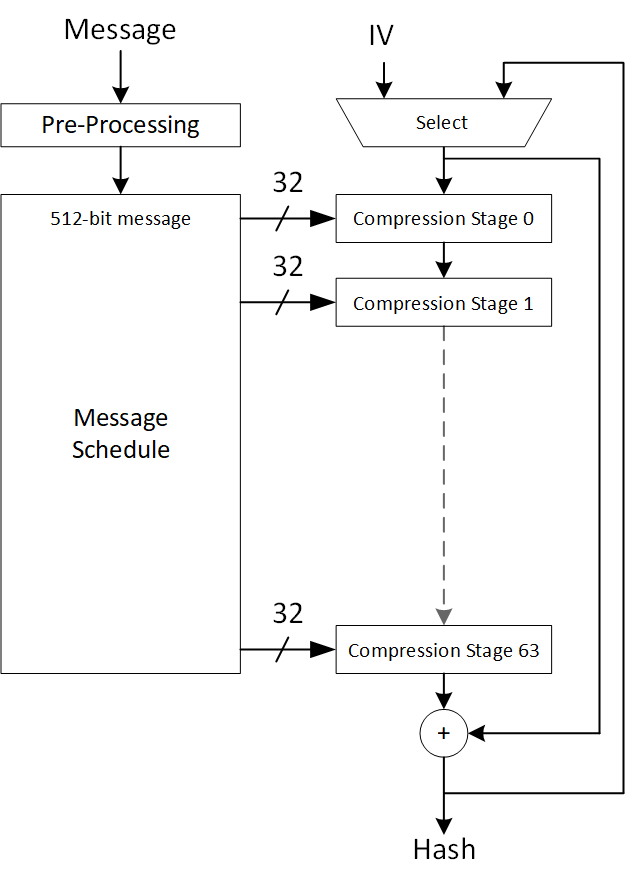
\includegraphics[scale=0.7]{sha256.png}
  \caption{SHA-256 Block Diagram}
  \label{sha2.fig}
\end{figure}

The IV in Figure~\ref{sha2.fig} is called the Initialization Vector
and we are not using it in this laboratory.  The IV is commonly
used in cryptographic systems to give another layer of security to
systems.  For example, when
you use your credit card and are asked to put in your pin to complete a purchase.

\subsection{ASCII}

ASCII stands for American Standard Code for Information
Interchange. Computers can only understand numbers, so an ASCII code
is the numerical representation of a character such as 'a' or '@' or
an action of some sort. ASCII was developed a long time ago and now
the non-printing characters are rarely used for their original
purpose. Table~\ref{ascii.tbl} is an abbreviated
ASCII character table. ASCII was
actually designed for use with teletypes, so the descriptions are
somewhat obscure.
ASCII has expanded for other uses, however, its use is still
utilized as it is easy to use for the english alphabet (sometimes being
called US-ASCII).
ASCII has just $128$ code points, of which only $95$ are printable
characters, which severely limit its scope.  However, this has been
expanded to handle other alphabets.  More elaborate ASCII tables can
be found here: \url{https://en.wikipedia.org/wiki/ASCII}.

You will need to convert your text that you want to create a hash for
with ASCII codes.  You can either look it up manually using
Table~\ref{ascii.tbl} or use the included Python file to convert it
automatically.  Use these hex values to include in your SV
manually that will generate the hash value appropriately.  
\begin{table} [t!]
  \centering
  {\small
  \begin{tabular}{|c|c|c||c|c|c||c|c|c||c|c|c||c|c|c||c|c|} \hline
    Dec & Hex & Char & Dec & Hex & Char & Dec & Hex & Char & Dec & Hex & Char & Dec & Hex & Char\\ \hline \hline
    048 & 0x30 & 0 & 064 & 0x40 & @ &  080 & 0x50 & P        & 096 & 0x60 & \textquoteleft & 112 & 0x70 & p        \\ \hline
    049 & 0x31 & 1 & 065 & 0x41 & A &  081 & 0x51 & Q        & 097 & 0x61 & a              & 113 & 0x71 & q        \\ \hline
    050 & 0x32 & 2 & 066 & 0x42 & B &  082 & 0x52 & R        & 098 & 0x62 & b              & 114 & 0x72 & r        \\ \hline
    051 & 0x33 & 3 & 067 & 0x43 & C &  083 & 0x53 & S        & 099 & 0x63 & c              & 115 & 0x73 & s        \\ \hline
    052 & 0x34 & 4 & 068 & 0x44 & D &  084 & 0x54 & T        & 100 & 0x64 & d              & 116 & 0x74 & t        \\ \hline
    053 & 0x35 & 5 & 069 & 0x45 & E &  085 & 0x55 & U        & 101 & 0x65 & e              & 117 & 0x75 & u        \\ \hline
    054 & 0x36 & 6 & 070 & 0x46 & F &  086 & 0x56 & V        & 102 & 0x66 & f              & 118 & 0x76 & v        \\ \hline
    055 & 0x37 & 7 & 071 & 0x47 & G &  087 & 0x57 & W        & 103 & 0x67 & g              & 119 & 0x77 & w        \\ \hline
    056 & 0x38 & 8 & 072 & 0x48 & H &  088 & 0x58 & X        & 104 & 0x68 & h              & 120 & 0x78 & x        \\ \hline
    057 & 0x39 & 9 & 073 & 0x49 & I &  089 & 0x59 & Y        & 105 & 0x69 & i              & 121 & 0x79 & y        \\ \hline
    058 & 0x3A & : & 074 & 0x4A & J &  090 & 0x5A & Z        & 106 & 0x6A & j              & 122 & 0x7A & z        \\ \hline
    059 & 0x3B & ; & 075 & 0x4B & K &  091 & 0x5B & [        & 107 & 0x6B & k              & 123 & 0x7B & \char`\{ \\ \hline
    060 & 0x3C & < & 076 & 0x4C & L &  092 & 0x5C & \char`   & 108 & 0x6C & l              & 124 & 0x7C & |        \\ \hline
    061 & 0x3D & = & 077 & 0x4D & M &  093 & 0x5D & ]        & 109 & 0x6D & m              & 125 & 0x7D & \char`\} \\ \hline
    062 & 0x3E & > & 078 & 0x4E & N &  094 & 0x5E & \^{}     & 110 & 0x6E & n              & 126 & 0x7E & \~{}     \\ \hline
    063 & 0x3F & ? & 079 & 0x4F & O &  095 & 0x5F & \char`\_ & 111 & 0x6F & o              & 127 & 0x7F & \DEL     \\ \hline
  \end{tabular}
  }
  \caption{Common English ASCII Characters}
  \label{ascii.tbl}
\end{table}


\subsection{Preprocessing}
\label{padding.sec}

Before the actual hash computation, the message $x$ has to be padded to
fit a size of a multiple of $512$ bit. For the internal processing, the
padded message must then be divided into blocks. This will be
dependent on the size of the message you plan on sending (e.g., SHA-256).

For example, assume that we have a message $x$ with a length of $l$
bits. To obtain an overall message size of a multiple of $512$ bits, we
append a single “1” followed by $k$ zero bits and the binary $64$-bit
representation of $l$. Consequently, the number of required zeros $k$ is
given by
\begin{eqnarray*}
  k & = & 512 - 64 - 1 - l
\end{eqnarray*}

For example, the (8-bit ASCII) message “abc” has length $8 \times 3 = 24$,
so the message is padded with a one bit, then $448 - (24 + 1) = 423$
zero bits, and then
the message length (i.e., $64$), to become the $512$-bit padded
message.  This is illustrated in Figure~\ref{padding.fig}
\begin{figure}
  \centering
  \includegraphics[scale=0.4]{padding.png}
  \caption{Padding example for ``abc'' for a $512$-bit padded message~\cite{1250396}}
  \label{padding.fig}
\end{figure}

This can be done easily within SystemVerilog with bitswizzling as
indicated in Section~\ref{swizzle.sec}.
An example of this could be the following SV Hardware Descriptive
Language (HDL).
\begin{verbatim}
assign padded = {message, 1'b1, {zero_width{1'b0}},  {back_0_width{1'b0}}, MSG_SIZE};
\end{verbatim}
The key to this is computing each value correctly.  The
\verb!MSG_SIZE! should be the message length to correctly fill the
message size to $512$ bits.  This value of $512$ is specific to
SHA-256 and is different for other SHA variants (e.g., SHA-512).  The
padding process is part of the SHA-256 algorithm applying the
Merkle-Damg{\aa}rd construction that is used to build cryptographic hash functions
from a fixed-length compression function~\cite{10.5555/1721909}.


\subsection{Hash Computation}

The real advantage to using digital logic is that much of the
computation can be done in parallel.  That is, when one piece of logic
is being computed, another part can be done at the same time reducing
the total amount of time for the computation.  Software, on the other
hand, typically is slower as it requires waiting for previous
operations to complete before it can move forward.

\subsubsection{Modular Addition}
\label{modular.sec}

The computation of the hash function is a combination of rotations,
shifts, and additions.  Addition is tricky as it has to be done not to
exceed the size of the addition (in this case, since it is a block of
$32$-bits, then it should not exceed $2^{32}$ or modulo $2^{32}$.  This is
called modular arithmetic and can be summarized in the following equation.
\begin{eqnarray*}
  \mid X+Y \mid_m ~= \Biggl\{
   \begin{array}{@{}ll@{}}
      X+Y,      & \text{ if $X+Y < m$}  \\
      X+Y-m,    & \text{ if $X+Y \geq m$} 
   \end{array}
\end{eqnarray*}  
Modular arithmetic is key to many cryptographic algorithm.
Fortunately, for our implementation it is quite easy as we just have
to drop off the MSB since it is a modulo addition for a power of $2^n$.

\subsubsection{constants}
\label{constants.sec}

Before hash computation begins for each of the secure hash algorithms,
the initial hash value,
$H^0$, must be set. For SHA-256, the size and number of words in $H^0$
depends on the message digest size.  These words area obtained by
taking the first thirty-two bits of the fractional parts of the square
roots of the first eight prime numbers to ensure the numbers are
random.  That is, the fractional parts of the square root of the following numbers
$2, 3, 5, 7, 11, 13, 17, 19$ (e.g., $\sqrt{2} = 1.414213562373090488016887
\rightarrow 0.414213562373090488016887$ which is equal to (more or less)
\verb!0.01101010000010011110011001101000! in binary).
These value are different for different versions of the Secure
Hash Standard (e.g., SHA-384)~\cite{1250396}.
\begin{eqnarray*}
  H_0^0 & = & \verb!0x6a09e667!\\
  H_1^0 & = & \verb!0xbb67ae85!\\
  H_2^0 & = & \verb!0x3c6ef372!\\
  H_3^0 & = & \verb!0xa54ff53a!\\
  H_4^0 & = & \verb!0x510e527f!\\
  H_5^0 & = & \verb!0x9b05688c!\\
  H_6^0 & = & \verb!0x1f83d9ab!\\
  H_7^0 & = & \verb!0x5be0cd19!\\
\end{eqnarray*}

There are some additional constants utilized within the main hash
computation.  These are computed similar based on the cube roots of
the first sixty-four prime numbers and labeled
$K_0^{256}, K_1^{256}, \ldots K_{63}^{256}$, as shown here.
\begin{verbatim}
428a2f98 71374491 b5c0fbcf e9b5dba5 3956c25b 59f111f1 923f82a4 ab1c5ed5
d807aa98 12835b01 243185be 550c7dc3 72be5d74 80deb1fe 9bdc06a7 c19bf174
e49b69c1 efbe4786 0fc19dc6 240ca1cc 2de92c6f 4a7484aa 5cb0a9dc 76f988da
983e5152 a831c66d b00327c8 bf597fc7 c6e00bf3 d5a79147 06ca6351 14292967
27b70a85 2e1b2138 4d2c6dfc 53380d13 650a7354 766a0abb 81c2c92e 92722c85
a2bfe8a1 a81a664b c24b8b70 c76c51a3 d192e819 d6990624 f40e3585 106aa070
19a4c116 1e376c08 2748774c 34b0bcb5 391c0cb3 4ed8aa4a 5b9cca4f 682e6ff3
748f82ee 78a5636f 84c87814 8cc70208 90befffa a4506ceb bef9a3f7 c67178f2
\end{verbatim}

These values are already given to you in the SV.  The trick is to make
sure you reference the correct value from the array.  For example, the
value of $H$ is given as:
\begin{verbatim}
 logic [255:0] H = {32'h6a09e667, 32'hbb67ae85,
		      32'h3c6ef372, 32'ha54ff53a, 32'h510e527f, 32'h9b05688c,
		      32'h1f83d9ab, 32'h5be0cd19};
\end{verbatim}
Therefore, to get $H_0^0$ you should  use \verb!H[255:224]!.  There are
some clever ways of indexing the values in this array, but I will
leave that up to you if you wish to explore them.

\subsubsection{Main SHA-256 computation}

SHA-256 in hardware is typically very easy if taken systematically.
For this laboratory, we will only use 1 $m$-bit block or 1 $512$-bit
block.  In theory, hardware may be composed of multiple blocks.  To
visualize this block, think about it as a huge ripple-carry adder (RCA)
where each block is passed to the next.

SHA-256 can be used to hash a message, $M$, having a length of $l$
bits, where $0 \leq l < 2^{64}$. The
algorithm uses 1) a message schedule of sixty-four $32$-bit words,
2) eight working variables of $32$
bits labeled $a$ through $h$, and 3) a hash value of eight $32$-bit words.
The final result of SHA-256 is a $256$-bit
message digest.
The words of the message schedule are labeled
$W_0, W_1, \ldots, W_{63}$. The
eight working variables are labeled $a$, $b$, $c$, $d$, $e$, $f$, $g$,
and $h$ and computed within each of the $64$ hash computation blocks.
The words of the hash value are labeled $H_0^i, H_1^i, \ldots H_7^i$.
which will hold the initial hash value, $H^0$, replaced by each
successive intermediate hash value
(after each message block is processed), $H^i$, and ending with the
final hash value, $H^N$.  For cryptographic systems, this is sometimes
called a round and is a common word utilized in these types of systems
to randomize inputs similar to shuffling a deck of cards.

The operation looks more complicated than it is but its just a series
of computations similar to the RCA in Lab 1.  The key is to get the order of
processing correct and, of course, the compute the correct number of steps.
A key piece item to remember is that
addition (+) is performed modulo $2^{32}$ as described in Section~\ref{modular.sec}.
\begin{enumerate}
  \item Preprocesssing: set the initial hash values $H^0$ as previously
    specified as well as the padding (see Section~\ref{padding.sec}).
  \item Prepare the message:
    \begin{itemize}
  \item Since we are only operating on $1$ group or $N=1$, we can
    break the computation down into blocks of $32$ for each part
    of the message and operate on the message for $64$ rounds (i.e.,
    $0 \leq t \leq 15$).
    That is, each message block, $M^1, M^2, \ldots, M^{64}$. 
    is processed in order.  We are only processing $1$ message for
    this laboratory, therefore, your message can not be bigger than
    $512$-bit message length.  
  \item For blocks $16 \leq t \leq 63$, we need to compute
    $W_t = \sigma_1^{256} (W_{t-2}) + W_{t-7} + \sigma_0^{256} (W_{t-15}) + W_{t-16}$
    where
    \begin{eqnarray*}
      \sigma_0^{256}(x) = \text{ror}^{7}(x) \oplus \text{ror}^{18}(x) \oplus (x~\verb!>>!~3)    \\
      \sigma_1^{256}(x) = \text{ror}^{17}(x) \oplus \text{ror}^{19}(x) \oplus (x~\verb!>>!~10)    
    \end{eqnarray*}
  \item This can be summarized as follows:
    \begin{eqnarray*}
      W_t = \Biggl\{
      \begin{array}{@{}ll@{}}
        M_t^i,      & (0 \leq t \leq 15)  \\
        \sigma_1^{256} (W_{t-2}) + W_{t-7} + \sigma_0^{256} (W_{t-15}) +  W_{t-16},  & (16 \leq t \leq 63) 
      \end{array}
    \end{eqnarray*}  
    
    \end{itemize}
    
    \item Initialize the seven working variables with the (i-1)st (see Section~\ref{constants.sec})
      hash.  For example, once the message is prepared in Step 2,
      $a = H_0^0$, $b = H_1^0$, and so on.  Each value of $a$ through
      $h$ will be an input into the next block of Step~$4$.  
      \begin{itemize}
      \item $a = H_0^{i-1}$
      \item $b = H_1^{i-1}$
      \item $c = H_2^{i-1}$
      \item $d = H_3^{i-1}$
      \item $e = H_4^{i-1}$
      \item $f = H_5^{i-1}$
      \item $g = H_6^{i-1}$
      \item $h = H_h^{i-1}$        
      \end{itemize}

    \item Compute the following items for $t = 0~\text{to}~63$ using      
      $T_1 = h + \Sigma_1^{256} (e) + \text{Choice}(e,f,g) + K_t^{63} + W_t$ and
      $T_2 = \Sigma_0^{256} (a) + \text{Majority}(a,b,c)$.  These 
      equations are broken down as for $\Sigma_1$, $\Sigma_0$
      and $\text{Choice(x,y,z)} = (x \cdot y) \oplus (\overline{x} \cdot z)$ and
      $\text{Majority(x,y,z)} = (x \cdot y) \oplus (x \cdot z) \oplus (y
      \cdot z)$.  The \verb!Majority! and \verb!Choice! functions are
      actually ternaries similar to what we learned in class with a
      multiplexor.
      The values of $\Sigma_1^{256}$ and $\Sigma_0^{256}$
      are similar to the lower case versions above.  That is, it
      is only composed of xor and ror operations (i.e., there are no right shifts).
      \begin{eqnarray*}
        \Sigma_0^{256}(x) = \text{ror}^{2}(x) \oplus \text{ror}^{13}(x) \oplus \text{ror}^{22}(x)    \\
        \Sigma_1^{256}(x) = \text{ror}^{6}(x) \oplus \text{ror}^{11}(x) \oplus \text{ror}^{25}(x)    
      \end{eqnarray*}
  \begin{itemize}
  \item $h = g$
  \item $g = f$
  \item $f = e$
  \item $e = d + T_1$
  \item $d = c$
  \item $c = b$
  \item $b = a$
  \item $a = T_1 + T_2$
  \end{itemize}
  This block is done $64$ times and each value of $a$-$h$ is passed to the
  next block (e.g., The output $a$ will be the next value of $H_0^1$
  from Step~$3$.  Figure~\ref{sha256compression.fig} shows a visual idea
  of what this step is accomplishing and is sometimes called a compression function
  - again, it is performed $64$ times.
  \begin{figure} [t!]
  \centering
  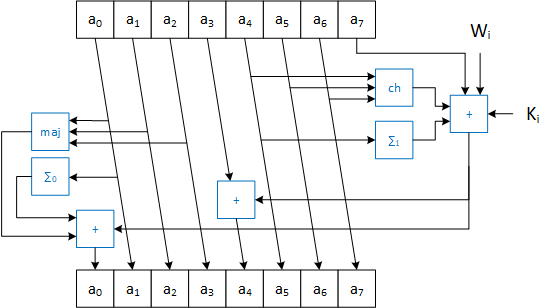
\includegraphics[scale=0.8]{sha256compression2.png}
  \caption{SHA256 Compression Function Block}
  \label{sha256compression.fig}
  \end{figure}
  
  \item After processing $64$ blocks from Step~$4$, add the working
    variables above to the current hash variable    
    to the current variables.
    \begin{itemize}
    \item $H_0^1 = a + H_0^0$
    \item $H_1^1 = b + H_2^0$
    \item $H_2^1 = c + H_3^0$
    \item $H_3^1 = d + H_3^0$
    \item $H_4^1 = e + H_4^0$
    \item $H_5^1 = f + H_5^0$
    \item $H_6^1 = g + H_6^0$
    \item $H_7^1 = h + H_7^0$
    \end{itemize}

  \item Finally, concatenate or squish all the values in the
    previous step together forming a $512$-bit message (i.e., $32$
    hexadecimal digits).
    \begin{eqnarray*}
      \{H_0^1 || H_1^1 || H_2^1 || H_3^1 || H_4^1 || H_5^1 || H_6^1 || H_7^1\}
    \end{eqnarray*}
    
\end{enumerate}


\subsection{Power, Performance and Area (PPA)}

For this laboratory, we are going to analyze the design with better
PPA.  That is, you should analyze your design for Power, Performance
and Area.  As opposed to previous laboratories, this procedure that
will be documented here is more robust and gives better numbers that
you can use to assess whether your design is credible or not.  As with
any digital design, engineers use PPA to assess the level of
difficulty, challenge, and effort needed for a design.

To assess your PPA for this design, you should determine its PPA after
implementation.  This is because some of the PPA results (e.g.,
timing) are not adjusted properly until the Implementation phase.  The
Implementation phase typically places and routes the design onto the
FPGA by connecting all the logic blocks that we read about in the
article that we looked at in Lab 0~\cite{7086413}.

To obtain the PPA results, you first have to run through your design
making sure that it is implemented correctly.  Then, you need to add
the following reports after the route stage (i.e., during
Implementation):
\begin{enumerate}
\item \verb!report_utilization! : Area
\item \verb!report_timing! : Performance
\item \verb!report_power! : Power
\end{enumerate}
You can the reports you need by clicking on the reports tab, right
mouse clicking, and then adding the report you need, as shown in
Figure~\ref{reports1.png}.  Once you add the report, it is easiest to
re-run the implementation to get the report.  Clicking on the option
gets you specific report which you can save.
\begin{figure} [b!]
  \centering
  \includegraphics[scale=0.3, width=\columnwidth]{analysis.png}
  \caption{Reports Window within Xilinx Vivado}
  \label{reports1.png}
\end{figure}

  
\section{Tasks}

Most of the blocks and their operation
have been given to you to help you understand the
problem better.
For those that are interested in more about cryptography and how
hardware can impact the future, I encourage you to read more about it
through searching on the Internet as well as this great
reference~\cite{10.5555/1721909}.
One of the hard parts of any engineering problem is
to understand what is going on and making sure you are correct.  This
will be quite apparent within this laboratory.

To make things go
smoothly, I encourage you to understand how the algorithm works first.
Digital designers rely heavily on getting good \textit{known} data to make
sure what their logic produces is correct.  Typically, this is done
either on paper and
pencil or through software.  My main goal for this laboratory is give
you a good experience in debugging while giving you a challenge for
implementing an interesting and complex piece of combinational logic.

We will use software for our verification in this laboratory 
using some software written in Python.  Python is now rated the
number one programming language by the IEEE and the ACM.  I encourage
you to learn more about Python, as it is utilized quite extensively in
current commercial systems.
If you need to install Python on your home machine or laptop, go to
Microsoft Store and install \verb!python3! (latest version 
is \verb!Python 3.12.5! as of 9/24/24).
You can also use the following URL
\url{https://www.python.org/downloads/windows/}
and download the appropriate version.

The main Python output is quite verbose, but it should be available in
your \verb!python! subdirectory of your repository.  To run the program,
navigate to this \verb!python! subdirectory and type
\verb!python3 sha256.py!.  It will output a ton of information for
each step in hexadecimal listed above you can use for debugging and
verification.  The
key in this laboratory or any complex digital system
is to take things slowly and debug things step by step first.  

Verification is extremely difficult
because there are so many moving parts.  Use the
Python program to verify each block out of the HDL.  There is also some
great web pages that can be used to verify your design at
\url{http://sha256algorithm.com} and
\url{https://stepansnigirev.github.io/visual-sha256/}, as well.
\begin{figure} [t!]
  \centering
  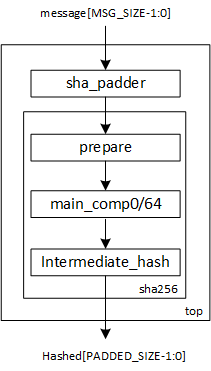
\includegraphics[scale=0.9]{sha256-block.png}
  \caption{Basic block diagram of your final SHA-256 (\texttt{sha256.sv})}
  \label{sha256-block.fig}
\end{figure}

The main tasks for this laboratory
will be the following elements:
\begin{enumerate}
  \item Design the SHA-256 combinational block for generating the hash
    in SystemVerilog and simulate with ModelSim.  A basic block
    diagram of what your final SV design should be using the naming convension
    found in your stubbed SV code is shown in
    Figure~\ref{sha256-block.fig}.  
    stubbed SV design.
  \item Use the Python output of \verb!sha256.py!
    or the following web page to help you with verifying the
    correct operation within ModelSim.
    There is also a decent online
    SHA-256 calculator available
    at \url{https://stepansnigirev.github.io/visual-sha256/} that
    shows some good input/output values to help validate a given block.
    Again, you should use whatever you feel comfortable with and
    helps you debug your implementation.
  \item Generate and test at least $5$ random messages and their respective hash generation
    using the testbench.
  \item After verifying your design with a testbench in ModelSim,
    implement your design on the DSDB board and use the    
    $7$-segment display to display your message and the resulting hash.
    Since you only have four $7$-segment displays, you will not be
    able to show the entire message, so you will
    have to figure a way to verify the operation.
  \item Use the push buttons, switches, and LEDs to help you input
    your message as well as debug operation and prove that your
    design works on your DSDB board.
    \item You should also analyze the PPA impact on your design. 
\end{enumerate}
This laboratory should involve \textbf{only combinational logic} and be
straight forward in creating Boolean logic with SystemVerilog.
Again, there are many parts to this design and based on experience, I
believe it will be easier to debug the items in small steps and then
once this works, debug the next step.  The message preparation and
padding are slightly easier than operations like the hash computation,
so it will optimize your design process if you focus on this block
first.  However, I would use the strategy that works the best for you.

\subsection{Testing and Stubbing Code}

You should use the testbenches you utilized for Lab0 and Lab1 to help
you test your design.  The design is completely combinational and
should not be any different in terms of structure than both of these
labs.  You can design the testbench to read in different messages to
automate the process as we did in Lab~$1$.

I have also given you some freebies to help you with this lab.  When
writing HDL or software, it is sometimes useful to \textit{stub} your
code.  A stubbed piece of code is a blank piece of software that has
most of your functions you believe will work for your design.
Fortunately, I have stubbed out your SV for you and you can use this
as a guide.  However, the design is up to you and you can change it if
you think it will help you optimize your design more effectively.
I also put some comments in the SV to help you know where
to instantiate certain items.

\subsection{Getting to know ModelSim and Debugging more in depth}

ModelSim is a professional Hardware Descriptive Language tool for
simulation and verification.  It has many neat features to help you
with debugging.  Although testbenches are the main vehicle for
understanding how to test a digital system, using ModelSim can save
you hours and days in debugging a design.  Therefore, we are also
going to introduce some new features of ModelSim that you should use
to help you with this laboratory. I also encourage you to use the
testbench skills you learned from Lab 1.

The features you will use in ModelSim are the \textit{Sim} and
\textit{Objects} window.  Normally both of these windows are present
when running a DO file, however, sometimes I find that they do not
open properly.  You may need to activate them in the View menu at the
top of ModelSim.  They should look like Figure~\ref{modelsim.png} when
activated.  Both of these windows are utilized with the Wave window.
\begin{figure} [t!]
  \centering
  \includegraphics[scale=0.3]{modelsim.png}
  \caption{ModelSim Sim and Objects Window}
  \label{modelsim.png}
\end{figure}

To use the two windows effectively, you should use the \textit{Wave}
to see the data at a certain time.  First, move your cursor to the
time you wish to investigate something - you should see a yellow line
indicating the time you are observing the data.  Next, you
should navigate to the
hierarchy of the module you wish to verify in the \textit{Sim} window
and the \textit{Objects} window will display all signals and values
that for that instance at a given time.  You might need to play around
with using these two windows together with the \textit{Wave} window,
but once you do you will find that its easy to debug what each block
is producing at a given time.

The "sim" window (orange) contains the hierarchy of the design.  The
top level shows the test bench (tb) with a expandable button to the
left.
By clicking the "+" it opens the hierarchy for all modules
instantiated in tb.  Clicking on the name of the instance changes
which objects (blue) are visible in the "objects" window.  You can
also add an
object to the wave by right clicking on the name of the object in the
"objects" window "Add Wave".  Your testbench and modules may use
different names but the same process applies to add signals to the
wave (purple).

You can save the wave by clicking in the wave window then clicking the
brown colored floppy disk icon in the toolbar.  (Third icon from the
left)  The saved file only contains the configuration of the wave not
the actual data. This allows you to recall the wave if you restart
modelsim at a later time.  To recall the wave you can type "do <name
of wave file> in the transcript (yellow).  You can also add this to
the do file so it always pulls up your wave every time the simulation
is run.

Modelsim has many extra features which can greatly aid in your debugging.
First let's discuss some tips and tricks.
\begin{itemize}
\item  If the toolbar gets disorderly, right click in the toolbar and
  select reset.
\item Signals in the wave by default show the full path name.  This can
  be changed to just the lowest level of hierarchy by clicking the
  ``toggle leafs name'' button in the lower left of the wave shown in
  Figure~\ref{modelsim-tips1.png}  
\item Zoom buttons are confusing.  The ``+'' zoom in is mostly useless.
  Use the yellow upside down ``T'' with magnifying glass to zoom in
  at the cursor, as shown in Figure~\ref{modelsim-tips2.png} in red.
\item The ``-'' zoom button works as expected.
\item If you select a signal in the wave viewer, ``Tab'' and ``Shift + Tab''
  will move the cursor to the next transition.
\item A multi-bit bus can be searched for a specific value using the ``Search''
  buttons in the toolbar.  The blue left and right allows to the right of
  the ``Search'' button will search backwards (left) or forwards (right)
  in time, as shown in Figure~\ref{modelsim-tips2.png} in green.
\end{itemize}

At the risk of complicating things the ``data flow'' window can be very
helpful when debugging red X's.  Either in the objects window or the wave
window right click a signal and select ``Add to dataflow''. This opens
a new window where you can right click and select ``ChaseX'' or ``TraceX''.
These allow you to quickly find the source of an X.  If this does not make
sense you can skip.
\begin{figure} [t!]
  \centering
  \includegraphics[scale=0.4]{modelsim-tips1.png}
  \caption{ModelSim toggle leafs. In the red box, the left-most box is the ``Now'' row.}
  \label{modelsim-tips1.png}
\end{figure}
\begin{figure} [t!]
  \centering
  \includegraphics[scale=0.32]{modelsim-tips2.png}
  \caption{Search inside the green box and zoom controls in the red box.}
  \label{modelsim-tips2.png}
\end{figure}

\subsection{Extra Credit}

If you get done early, you can attempt some extra credit.  However, I
would only try this option if you get everything verified within your
design.  
One possible improvement is to work on optimizing the verification
of your design.  You can do any other modification (e.g., re-writing
the Python code) or implementing SHA-512, as well.  By the way, once
you get SHA-256 working, it should not be difficult to extend to
SHA-512.

\subsection{Sources on the Internet}

This laboratory is unique to Oklahoma State University and I am not
oblivious that there are other implementations out there on GitHub.
You are welcome to look at these, but I encourage you to do your own
work.  It is not a bad idea to see what others design with HDL, but I
have been
designing HDL for a long time and I know when something is bad (most
often, copied from the Internet) and/or not your own work.  It is your job
to learn from this laboratory to become the awesome engineer that I know
you can become.  Copying from others is just a bad solution and does
not get you anywhere nor does it help you learn the material.
Therefore, please make sure you to do your own
work here!


\section{Submission}

You should electronically hand in your HDL (all files that you want
us to see) into Canvas.  You should also take a printout of your waveform 
from your ModelSim simulation.  Only one of your team members should upload
the files and/or lab report. Please contact James Stine
(james.stine@okstate.edu) 
for more help.  Your code should be
readable and well-documented. In addition, please turn in additional
test cases or any other added item that you used. 
Please also remember to document everything in your Lab Report using
the information found in the Grading Rubric.


    
\bibliographystyle{IEEEbib}
\bibliography{lab2}

\end{document}
